\documentclass[a4paper, 12pt, titlepage]{article}

\usepackage{graphicx, color} %for å inkludere grafikk
\usepackage{verbatim, color} %for å inkludere filer med tegn LaTeX ikke liker. \verbatiminput{verb.txt}
%\usepackage{gensymb} %gensymb Symbols Defined to Work in Both Math and Text Mode 

\usepackage[T1]{fontenc} %for å bruke æøå. upgrades to 256 bit encoding. More characters
\usepackage[utf8]{inputenc} %Kan forandres til latin1. utf8 gir norske tegn
%inputenc allows the user to input accented characters directly from the keyboard;
%fontenc is oriented to output, that is, what fonts to use for printing characters.
%\usepackage[norsk]{babel} 

\usepackage{pdfpages} %Importing external pdf-pages
\usepackage[compact]{titlesec} %Spacing for two-column document

\usepackage{textcomp} % make degrees centigrade symbols, euros, etc
\usepackage{amsmath, amssymb} %e.g. \begin{theorem}[Pythagoras], \begin{proof} or {align}
\usepackage{amsbsy, amsfonts} %\pmb for annerledes boldfont
\usepackage{parskip} %Space between paragraphs
\usepackage{float} %Im­proves the in­ter­face for defin­ing float­ing ob­jects such as fig­ures and ta­bles.
\usepackage{simplewick}
\usepackage{libertine} 
\usepackage{siunitx} % SI units. Example: \SI{100}{\micro\meter}

\usepackage{geometry} % Definerer marger. 
 %\geometry{headhight=1mm}
 \geometry{top=20mm, bottom=20mm, left=30mm, right=30mm} % Marger i mm. Total bredde er 210mm



\author{Wilhelm Holmen}
\title{FYS4411 Project 3}

\begin{document}
 \maketitle
 \newpage

 \tableofcontents

 \newpage

\begin{subsection}*{Abstract}
 Solving the Schrodinger equation analytically has not yet been done for atoms larger than Hydrogen. I have in this project looked at Monte Carlo integration with the Metropolis-Hastings algorithm to find the ground state energy for Helium, Beryllium and Neon. I used hydrogen-like wavefunctions with two variational parametres. There are different methods to achieve better results and I have looked more closely at the inclusion of a Padé-Jastrow factor, Importance sampling and Gaussian type orbitals. I use method of steepest descent and results from a Hartree-Fock calculation to find optimal values of the parametres. We produce energies that does not quite suffice to predict bounding energies in molecules, but will a reasonable estimation to the ground state energy. 
\end{subsection}

\begin{section}{Introduction}
 In this project I first give a brief introduction to some of the important parts of quantum mechanics. I will introduce the hydrogen-like wavefunctions, and the form of the Hamiltonian for larger atoms. I will also comment on the variational principle and the Hatree-Fock method. \par
 An important part of the variational monte carlo algorithm is choosing a good trial wave function. As explained in the section on variational principle, we will find the best approximation to the ground state energy by finding the best approximation to the wavefunction. In this section I will introduce the Slater determinant form on the wavefunction, the Padé-Jastrow factor and the final form of my wavefunctions. I will also give a brief introduction to the Gaussian type orbitals I have used. 
\end{section}

\begin{section}{Quantum mechanics}
 The goal of this project is to calculate the ground state energy for three different atoms. The Helium atom, the Beryllium atom and the Neon atom. The energy in a quantum mechanical system is found by solving the time-independent Schrodinger equation for the system. 
 \begin{align}
 	\hat H \left| \Phi \right> = E \left| \Psi \right>
 \end{align}
 There are many solutions to this eigenvalue equation, and we are looking for the lowest possible value for $E$, i.e. the ground state energy $E_0$. The Hamiltonain is given as the total energy operator
 \begin{align}
 	\hat H = \hat T + \hat V
 \end{align}
 where $\hat T$ is the kinetic energy operator, and $\hat V$ is the operator for potential energy. Note that we are mostly computing ratios, so the factors in front of wavefunctions are often neglected. 

 \begin{subsection}{The Hydrogen atom}
 The Hydrogen atom has a Hamiltonian on the form. 
 \begin{align}
 	\hat H = \hat T + \hat V = -\frac{\hbar^2}{2m} \nabla^2 - \frac{e^2}{4 \pi \epsilon_0 r} 
 \end{align}
 In this project, we will use atomic units for all calculations. If we want the energies given as electronvolts, we must multiply our results with $2E_0$, where $E_0 = 13.6$eV. The Hamiltonian in atomic units reads
 \begin{align}
 	\hat H = -\frac{\nabla^2}{2} - \frac{1}{r}
 \end{align}
 The Hydrogen atom is a system we can solve analytically. We will use the results from these calculations as a starting point when we are looking at larger atoms. The energies are given as
 \begin{align}
 	E_n = -\frac{1}{2n^2}
 \end{align}
 The wavefunctions are given as a product of a radial function and the spherical harmonics 
 \begin{align}
 	\Psi = R(r)P(\theta)F(\phi)
 \end{align}
 These results show that we get different energy states given as the 1s-state, 2s-state, 2p-state, 3s-state, etc, with their respective quantum numbers, n, l, m. We get the following results for the first two states
 \begin{align}
 	\phi_{1s} &= \phi_{100}(\vec r_i) = e^{-ar_i} \\
 	\phi_{2s} &= \phi_{200}(\vec r_i) = (1 - \alpha r_i/2) e^{-\alpha r_i / 2} 
 \end{align}
 The spherical harmoics $Y_{l ml} = P(\theta)F(\phi)$ are given as
 \begin{align}
 	Y_{00} &= \sqrt{\frac{1}{4 \pi}} \\
 	Y_{10} &= \sqrt{\frac{3}{4 \pi}} \cos(\theta) \\
 	Y_{1\pm1} &= \sqrt{\frac{3}{8 \pi}}\sin{\theta} e^{\pm i \phi}
 \end{align}
 We see that for the 2p-states we can no longer neglect the spherical harmonics because they are no longer a constant factor. We can introduce solid harmonics to represent write this angular dependence with cartesian coordinates. We get the following states
 \begin{align}
 	\phi_{20-1}(\vec r_i) &= \alpha z e^{-\alpha r_i / 2} \\
 	\phi_{200}(\vec r_i) &= \alpha y e^{-\alpha r_i / 2} \\
 	\phi_{201}(\vec r_i) &= \alpha x e^{-\alpha r_i / 2} 
 \end{align}
 \end{subsection}

 \begin{subsection}{The Helium atom}
  The Hamiltonian for the Helium atom is given as
  \begin{align}
  	\hat H = \hat T + \hat V = -\frac{\nabla_1^2}{2} -\frac{\nabla_2^2}{2} - \frac{2}{r_1} - \frac{2}{r_2} + \frac{1}{|r_1 - r_2|}
  \end{align}
  Where the last term represents the electron-electron-repulsion. This term is the reason the Helium atom is much more complicated than the Hydrogen atom. We have a three-body problem instead of a two-body problem. We will later in the project use the notation $r_{12} = |r_1 - r_2|$.
 \end{subsection}

 \begin{subsection}{The variational principle}
 	In this project the variational principle is very important. It simply states that for any wavefunction $\left| \Psi \right>$, the ground state energy is higher than the exact ground state energy. 
 	\begin{align}
 		\left< \Psi \right| \hat H \left| \Psi \right> \leq \left< \Psi_{exact} \right| \hat H \left| \Psi_{exact} \right> = E_{gs}
 	\end{align}
 	This means that no matter what wavefunction we choose, we will always be above or equal to the exact energy. That means we can find the variational parametres that minimizes our expectation value since the lower energy we find, the closer we are to the true value.
 \end{subsection}

 \begin{subsection}{Hartree-Fock calculations}
 	
 \end{subsection}

\end{section}
\newpage






\begin{section}{The trial wavefunction}
  We are looking for a solution to the time independent Schrodinger equation
  \begin{align}
  	\hat H \left| \Phi_0 \right> = E_0 \left| \Psi_0 \right>
  \end{align}
  However, we do not have the exact ground state wavefunction. We will therefore guess on a wavefunction for our system. We call this a trial wavefunction, $\left| \Psi_T \right>$. Keeping the variational principle in mind, we can let this wavefunction depend on a variational paramater, $\alpha$. By varying, $\alpha$, we are looking for the minimum value of the function
  \begin{align}
  	E_0 = \left< \Psi_T(\alpha) \right| \hat H \left| \Psi_T(\alpha) \right> 
  \end{align}
  Any many-particle wave function can be written as a linear combination of single particle wave functions.
  \begin{align}
  	\left| \Psi \right> = \sum_i c_i \left|phi_i \right> 
  \end{align}
  and when we want an ansatz for the trial wavefunction, we usually choose which single particle wavefunctions we want to work with. This is because we can get a nice closed-form solutions for each of the one-particle energies
  \begin{align}
  	\hat h_i \left| \phi_i \right> = \epsilon_i \left| \phi_i \right>	
  \end{align} 
  In this project I have done the calculations for two different one-particle wavefunctions. Namely the Hydrogen orbitals and Gaussian-type orbitals. 

  
 \begin{subsection}{The Slater determinant}
  When we want to make a general ansatz for the ground state wavefunction for a multi-particle wavefunction, we normally represent it by a slater determinant. 
  \begin{align}
  	\left| \Psi \right>_{SD} = \frac{1}{\sqrt{N!}}\left| \begin{matrix}
  		 							 \phi_1 (r_1)  &  \phi_1 (r_2)  & ... &  \phi_1 (r_N)  \\
  		 							 \phi_2 (r_1)  &  \phi_2 (r_2)  & ... &  \phi_2 (r_N)  \\
  		 							.. & .. & .. & .. \\
  		 							 \phi_N (r_1)  & \phi_N (r_2)  & ... &  \phi_N (r_N)  
  	                            \end{matrix} \right|
  \end{align}
  This way of writing the wave function satisfies the Pauli principle, because of the sign change due to a change in particles. 
  This Slater as written is zero since the spation wave functions for the spin up and spin down states are equal. We can rewrite the Slater determinant into a product of two smaller Slater determinants. One for spin up and one for spin down. Taking Beryllium as an example
  \begin{align}
  	\left| \Psi \right>_{SD} = \left| \begin{matrix}
  		 							 \phi_{100 \uparrow} (r_1)  &  \phi_{100 \uparrow} (r_2)  & \phi_{100 \uparrow} (r_3) &  \phi_{100 \uparrow} (r_4)  \\
  		 							 \phi_{100 \downarrow} (r_1)  &  \phi_{100 \downarrow} (r_2)  & \phi_{100 \downarrow}(r_3) &  \phi_{100 \downarrow} (r_4)  \\
  		 							\phi_{200 \uparrow} (r_1)  &  \phi_{200 \uparrow} (r_2)  & \phi_{200 \uparrow} (r_3) &  \phi_{200 \uparrow} (r_4) \\
  		 							 \phi_{200 \downarrow} (r_1)  &  \phi_{200 \downarrow} (r_2)  & \phi_{200 \downarrow}(r_3) &  \phi_{200 \downarrow} (r_4) 
  	                            \end{matrix} \right|
  \end{align}
  It can be shown that this is equal to the product
  \begin{align}
  	\text{det}\uparrow(r_1,r_2) \cdot \text{det}\downarrow(r_3,r_4) 
  \end{align}
  where
  \begin{align}
  	\text{det}\uparrow(r_1,r_2) = \left| \begin{matrix}
  		\phi_{100 \uparrow} (r_1)  &  \phi_{100 \uparrow} (r_2) \\ \phi_{200 \uparrow} (r_1)  &  \phi_{200 \uparrow} (r_2)
  	\end{matrix} \right|
  \end{align}
  and
  \begin{align}
  	 \text{det}\downarrow(r_3,r_4) = \left| \begin{matrix}
  	 	\phi_{100 \downarrow}(r_3) &  \phi_{100 \downarrow} (r_4)  \\ \phi_{200 \downarrow}(r_3) &  \phi_{200 \downarrow} (r_4)
  	 \end{matrix} \right|
  \end{align}
  This ansatz is however not antisymmetric under the exchange of particles, but it will provide the same expectation value as the full Slater determinant. This splitting of the Slater determinant requires that the Hamiltonian is independent of spin and that we have an even number of particles. Both are fullfilled for this project. This splitting will also provide a small computational benefit because we will compute smaller determinants.
  \end{subsection}

 \begin{subsection}{Hydrogen orbitals}
  The hydrogen orbitals are the different eigenstates for the Hydrogen atom. We can make an ansatz for our trial wave function that use the lowest possible hydrogen orbitals as our one-particle wavefunctions. For helium, that means we fill up the two 1s-states. 
 \begin{figure}[H]
  	\centering
  	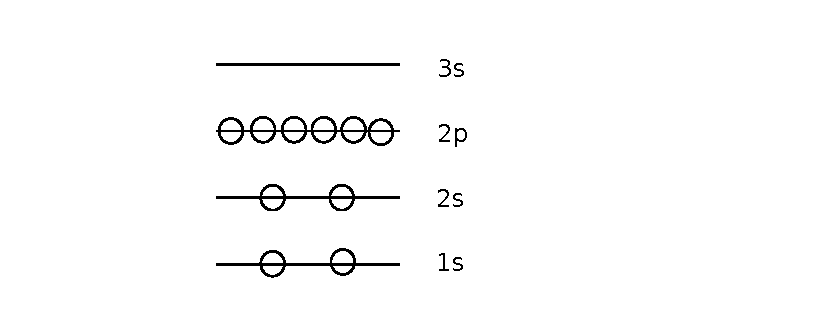
\includegraphics{orbitals.pdf}
  	\caption{Figure showing which hydrogen orbitals are occupied for Neon}
  \end{figure}
  If we disregard the interaction term in the Hamiltonian, this will give the exact result for the system. I have later used this to verify that the code produces the right energies. \par
  For Helium we get
  \begin{align}
  	\Psi_0 = \phi_{1s}(\vec r_1) \phi_{1s}(\vec r_2) \propto e^{-Z(r_1+r_2)} 
  \end{align}
  \begin{align}
  	E_0 = -\frac{Z^2}{2} - \frac{Z^2}{2} = -4
  \end{align}
  While Beryllium gives
  \begin{align}
  	E_{0, Be} = -2\frac{Z^2}{2} - 2 \frac{Z^2}{8} = -16 - 4 = -20
  \end{align}
  And ground state energy for Neon is $-200$. \par
  We cannot neglect the interaction between the electrons, so introduce a variational paramater $\alpha$ instead of the charge $Z$ in the exponent. Using the variational principle, we will vary this $\alpha$ until we get the lowest possible energy. 
 \end{subsection}
 \begin{subsection}{The Jastrow factor}
  As we will see later, the hydrogen orbitals is not a very good approximation to the ground state energy. We can take the interraction between the electrons into account in the wavefunction. This corrolation factor is known as the Padé-Jastrow factor and is on the form
  \begin{align}
  	\Psi_C = \prod_{i<j}^N e^{\frac{ar_{ij}}{1+\beta r_{ij}}}; \quad \quad r_{ij} = \left| \vec r_i - \vec r_j \right| 
  \end{align}
  Here $a=0.25$ if electron $i$ and $j$ have equal spin. Otherwise $a =0.5$. The Jastrow factor accounts for a small amount of the total energy. This is as expected because the interaction between the nucleus and the electrons are much stronger than the electron-electron repulsion. 
 \end{subsection}
 \begin{subsection}{Implemented wavefunctions}
  I have introduced two variational paramaters, namely $\alpha$ and $\beta$. For all three atoms, these are the parametres I will vary until I get the lowest possible energy. \par 
  Helium has two particles only, and splitting the Slater determinant results in two $1x1$ determinants, which can be written without the determinant sign. 
  \begin{align}
  	\Psi_T = \phi_{100 \uparrow}(\vec r_1) \phi_{100 \downarrow}(\vec r_2) \Psi_C(r12) = e^{-\alpha (r1+r2)} \text{exp}(\frac{r_{12}}{2(1+\beta r_{12})})
  \end{align}

  The Beryllium and Neon wave functions iare given by the spin-up and spin-down determinants defined above
  \begin{align}
  	\Psi_T = \text{det}\uparrow(r_1,r_2) \cdot \text{det}\downarrow(r_3,r_4) \prod_{i<j}^N e^{\frac{ar_{ij}}{1+\beta r_{ij}}}
  \end{align}
  where the Neon determinants are $5x5$ matrices given as
  \begin{align}
  	\text{det}\uparrow = \left| \begin{matrix}
	 	\phi_{100 \uparrow} (r_1)  &  \phi_{100 \uparrow} (r_2)  & \phi_{100 \uparrow} (r_3) &  \phi_{100 \uparrow} (r_4) & \phi_{100 \uparrow} (r_5) \\
		\phi_{200 \uparrow} (r_1)  &  \phi_{200 \uparrow} (r_2)  & \phi_{200 \uparrow} (r_3) &  \phi_{200 \uparrow} (r_4) & \phi_{200 \uparrow} (r_5) \\
		\phi_{21-1 \uparrow} (r_1)  &  \phi_{21-1 \uparrow} (r_2)  & \phi_{21-1 \uparrow} (r_3) &  \phi_{21-1 \uparrow} (r_4) & \phi_{21-1 \uparrow} (r_5) \\
		\phi_{210 \uparrow} (r_1)  &  \phi_{210 \uparrow} (r_2)  & \phi_{210 \uparrow} (r_3) &  \phi_{210 \uparrow} (r_4) & \phi_{210 \uparrow} (r_5) \\
		\phi_{211 \uparrow} (r_1)  &  \phi_{211 \uparrow} (r_2)  & \phi_{211 \uparrow} (r_3) &  \phi_{211 \uparrow} (r_4) & \phi_{211 \uparrow} (r_5) \\			
           	     \end{matrix} \right|
  \end{align}
 \end{subsection}

 \begin{subsection}{Gaussian type orbitals}
  Trying and testing for the best $\alpha$ is a crude and unprecise way of finding the optimal parameter. A better method to find the optimal wavefunction is by using a Hartree-Fock calculation. I have not done this in the project, but I have used the results from other calculations and implemented them. I have implemented this in addition to changing from the hydrogen orbitals to Gaussian type orbitals. This 

 \end{subsection}
\end{section}

\begin{section}{Variational Monte Carlo method}
   et teori avsnitt hvor du skriver kort om hva slags teorielement du har brukt (variasjonell MC, statistisk analyse med blocking, gradient metoder og soeking etter minima og mer), deretter

   As stated in the introduction, the point of the project is to solve the Schrodinger equation and find the ground state energy
   \begin{align}
   	\hat H \left| \Psi \right> = E \left|\Psi \right> 
   \end{align}
   This will be done by taking the expectation value of the Hamiltonian
   \begin{align}
   	\left< \Psi \right| \hat H \left| \Psi \right> = E[H] = \frac{\int d \mathbf{R} \Psi^*_T(\mathbf{R}) H(\mathbf{R}) \Psi_T(\mathbf{R})}{ \int d \mathbf{R} \Psi^*_T(\mathbf{R}) \Psi_T(\mathbf{R})}
   \end{align}
 	And from the variational principle, we know that 
 	\begin{align}
 		E[H] \geq E_{gs}
 	\end{align}
 	So the steps of this project is to choose a variational wavefunction, calculate the integral for $E[H]$ and minimize it with respect to the variational parametres. That is, we need to minimize the value
 	\begin{align}
 		E[H(\alpha, \beta)] = \frac{\int d \mathbf{R} \Psi^*_T(\mathbf{R},\alpha,\beta) H(\mathbf{R}) \Psi_T(\mathbf{R},\alpha,\beta)}{ \int d \mathbf{R} \Psi^*_T(\mathbf{R},\alpha,\beta) \Psi_T(\mathbf{R},\alpha,\beta)}
 	\end{align}
 	We define a new quatnity 
 	\begin{align}
 		E_L({\mathbf{R},\alpha,\beta}) = \frac{1}{\Psi_T(\mathbf{R},\alpha,\beta)} \hat H \Psi(\mathbf{R},\alpha,\beta)
 	\end{align}
 	And we see that by introducing the probability distribution
 	\begin{align}
 		P(\mathbf{R}) = \frac{|\Psi(\mathbf{R})|^2}{\int|\Psi(\mathbf{R})|^2 d \mathbf{R}}
 	\end{align}
 	We can write the total energy as
 	\begin{align}
 		E[H(\alpha,\beta)] = \int P(\mathbf{R},\alpha,\beta) E_(\mathbf{R},\alpha,\beta) d \mathbf{R} \approx \frac{1}{N} \sum_{i=1}^N P(\mathbf{R}_i,\alpha,\beta) E_L(\mathbf{R}_i,\alpha,\beta)
 	\end{align}
 	Where we calculate the local energy in each time and take the mean value. 

 \begin{subsection}{Metropolis algorithm}
 	The metropolis algorithm is a way to incorporate the probability distribution function in the calculation. The Metropolis algorithm is defined as following. We define $P_i^n$ as the probability of finding the system in the state $i$ at the step n. 
 	We now sample a possible new state $j$ with the probability $T_{i\to j}$. 

 	There is a probability $A_{i\to j}$ that we accept this new state, and $1-A_{i \to j}$ probability that we reject the move and use state $i$ again. 

 	We can show that 
	\begin{align}
 		\frac{A_{j\to i}}{A_{i\to j}} = \frac{p_i T_{i\to j}}{p_j T_{j\to i}}	
 	\end{align}
 	And the Metropolis choice is to maximize the A values, i.e. 
 	\begin{align}
 		A_{j \to i} = min\left( 1, \frac{p_i T_{i\to j}}{p_j T_{j\to i}} \right)
 	\end{align}
 	This will make sure that we integrate over the positions multiplied with the corresponding probability distribution, $P(\mathbf{R})$. 

 \end{subsection}

 \begin{subsection}{Importance sampling}
 	
 \end{subsection}

 \begin{subsection}{Statistical analysis}
 	A Monte Carlo simulation gives rise to two kinds of error. Systematic errors and statistical errors. Systematic errors are due to limitations of the applied models and faulty implementations. Here I will explore methods to estimate the statistical error. 

 Given a set of local energies, the variance is a measure of the spread from the true mean. The definition is
 \begin{align*}
 	\text{Var}(E) = \left< E^2 \right> - \left< E \right> ^2 
 \end{align*}
 Unfortunatly we do not know the true mean in a Monte-Carlo simulation. The computed average $\overline E$ is an approximation to the exact mean, and we do the following approximation
 \begin{align*}
 	\text{Var}(E) \approx \overline{E^2} - \overline{E}^2 
 \end{align*}
 For the case where we have the exact wave function, the variance becomes $0$, so the variance is an excellent measure of how close we are to the exact wave function. The variance however is \textit{not} a direct measure of the error. The standard deviation, the square root of the variance is related of the \textit{spread} in the sampled value. 
 \begin{align}
 	\sigma ^2(x) = \text{Var}(x)
 	\label{deviation}
 \end{align}
 This does not account for the samples being corrolated. Two samples, $x$ and $y$ are corrolated if the \textit{Covariance} is non-zero.
 \begin{align*}
 	\text{Cov}(x,y) = \left< xy \right> - \left< x \right> \left<y \right> 
 \end{align*}
 The diagonal elements of the Covariance is the Variance. By ignoring the corrolations, one get an error estimate that is generally too small. Given the true deviation, $\sigma_e$ and $\sigma$ from (\ref{deviation}) we have
 \begin{align*}
 	\sigma_c \geq \sigma
 \end{align*}

 The most interesting quantity when doing statistical analysis is not the error of single samples. It is the error of the mean value. One can show that the variance for the mean value, $m$ is 
 \begin{align}
 	\sigma^2 (m) = \frac{1}{n} \text{Cov}(x)
 	\label{covariance}
 \end{align}
 Where n is the number of samples used to calculate $m$ and 
 \begin{align*}
 	m = \frac{1}{n} \sum_i^n x_i
 \end{align*}
 Calculating the Covariance is an expensive process for a large sample set, so we need a better way to calculate this. 

 There is no need to do statistical analysis within the Monte-Carlo simulation. By storing the data set, one can estimate the error post process. An efficient algorithm for this is called blocking. 

 Given a set of $N$ samples from a single Monte-Carlo process. This set is divided into $n$ blocks of size $n_b = N/n$. Now we can treat each block as an individual simulation to calculate the variance of a calculated mean, $m$. This will in turn give us the covariance by (\ref{covariance}).
 \begin{align*}
 	\sigma^2 (m) = \left<m^2\right> - \left<m\right>^2 
 \end{align*}

 One can not know beforehand which block size is optimal to compute the exact error. One can, however, plot the variance against different block sizes. The curve should be stable over a span of block sizes. This plateau will serve as a reasonable approximation to the covariance. 
 \end{subsection}
 \begin{subsection}{One-body density}
 	The one-body density is defined as
 \begin{align*}
 	\rho(r_1) = \int_{r_2} .. \int_{r_N} | \Phi(r_1 r_2 .. r_N) |^2 dr_2 .. dr_N
 \end{align*}

 The distribution $|\Phi(r)|^2$ describes the distribution of a particle in the system. The one-body density $\rho(r_1)$ describes the simultaneous distribution of every particle in the system. $\rho(r_1) dr_1 $ represents the probability of finding \textit{any} particle in the volume element $dr_1$ as oppsed to $|\Phi(r)|^2$ giving the probability of finding \textit{particle $r_1$} in the volume element $dr_1$. Due to the indistinguishable nature of the particles, any of the coordinates contain information about all the particles. I will therefore normalize this density to the number of particles $N$ and not $1$ which is common for the one-particle density. 

 The way this is computed in a Monte Carlo simulation is by taking snapshots of all positions for every timestep, then constructing a histogram to construct an approximation to the wave function.

 The charge density for a single particle is given by 
 \begin{align*}
 	\rho_q (r) = q |\Psi(r)|^2
 \end{align*}
 However, since we already have computed the many-body probability density, we can use this instead to get the many-body charge density of the system. 
 \begin{align*}
 	\rho_q (r) = Q \rho(r_1)
 \end{align*}
 \end{subsection}

\end{section}

\begin{section}{implementation}
  * et implementasjon kapittel hvor du forteller hvordan du har implementert teorien, skriv om algo for SD, algo for Jastrow faktor, hvordan blocking er implementert samt testen du har brukt for aa verifisere koden. Her boer du baade diskutere hvordan du har testa analytisk lokal energi kontra numerisk derivasjon, liste cpu tidsbesparelse samt andre tester du har gjort, feks analytisk SD for beryllium kontra algoritmen for beryllium osv. Du trenger ikke liste heile koden her, det kan du legge til appendiks. 


  \begin{subsection}{Method of steepest descent}
  	Up until now, I have used measurment by eye to find the optimal values for $\alpha$ and $\beta$. This can be done in a more precise way, namely using methods like steepest descent or Conjugate Gradient method. I have included the steepest descent method in my project.
 If a function $F(x)$ is differentiable and in the neighborhood of a point $\mathbf{a}$, then the function $F(x)$ decreases fastest in the direction of the negative gradient, $-\nabla F(x)$. i.e. we are approaching a minima. Since the variational principle holds for $\left<\hat H\right> $, the best values for $\alpha$ and $\beta$ are the ones giving this minima. 
 \begin{align*}
 	\mathbf{b} = \mathbf{a} - \gamma \nabla F(\mathbf{a}) 
 \end{align*}
 if $\gamma$ is small enough, $F(\mathbf{b}) \leq F(\mathbf{a})$. We can therefore set up the scheme
 \begin{align*}
 	x_{n+1} = x_n - \gamma \nabla F(x_n)
 \end{align*}
 and continue until
 \begin{align*}
 	x_{n+1} - x_n \leq \text{precision}
 \end{align*}
  \end{subsection}


 \begin{subsection}{Finding optimal step length}
 	
 \end{subsection}
	
 \begin{subsection}{Performance optimizations}
  	
 \end{subsection}

\end{section}

\begin{section}{Results and discussion}

* resultater. Her kan du diskutere bla resultatene for He, be og Ne med de ulike approksimasjonene du har gjort, rekninger med bare SD og rekninger med baade SD og Jastrow. Hvor mye paavirker Jastrow faktoren resultatet for energien, er det forskjeller mellom He, be og Ne med tanke paa korrelasjoner, dvs spiller Jastrow faktoren like stor rolle for alle tre atomer osv. I tillegg boer du diskutere jastrow faktorens rolle naar du plotter en-partikkeltettheter og proeve aa trekke noen konklusjoner utifra det.


 \begin{subsection}{First look at Helium atom}
 	The first attempt at finding the ground state energy for Helium is found in the code for Project 1. figure (\ref{Helium1}) shows the variance and energy as we vary the parameter alpha. These results are without the Jastrow factor. 

 \begin{figure}[H]
 	\centering
 	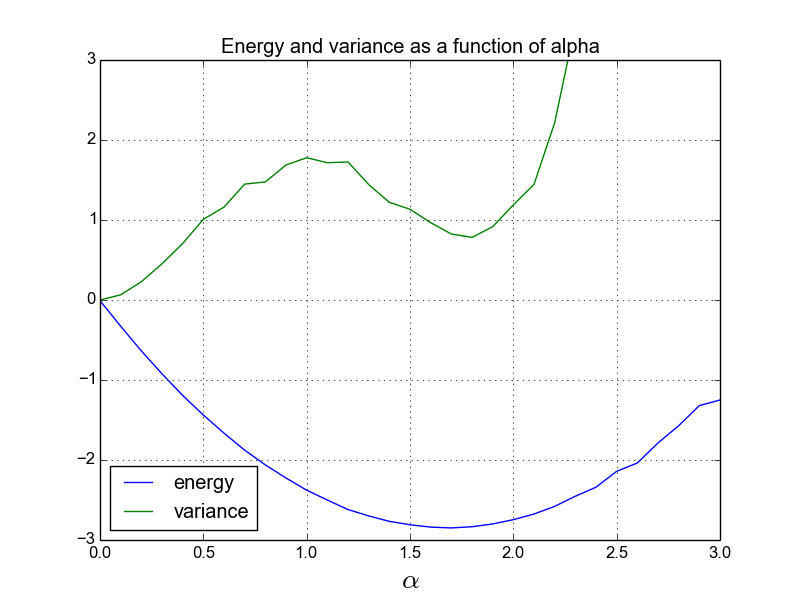
\includegraphics[width=0.8\textwidth]{../python_programs/EnergyVariance_helium1.png}
 	\label{Helium1}
 \end{figure}

 By looking closer at the energy and variance around $\alpha = 1.68$ in figure (\ref{Helium2}), we see that we get an energy of $\left<E\right> = -2.84997$, with a variance of $\sigma ^2 = 0.932912$. This is too far off from the best experimental value of $E_{experimental} = -2.903$. We see however that the variance is smaller for $\alpha = 1.8$, $1.9$ and $1.6$. But by the variational principle, we want as low energy as possible, so we choose the best $\alpha$ as $1.68$. 
 
 \begin{figure}[H]
 	\centering
 	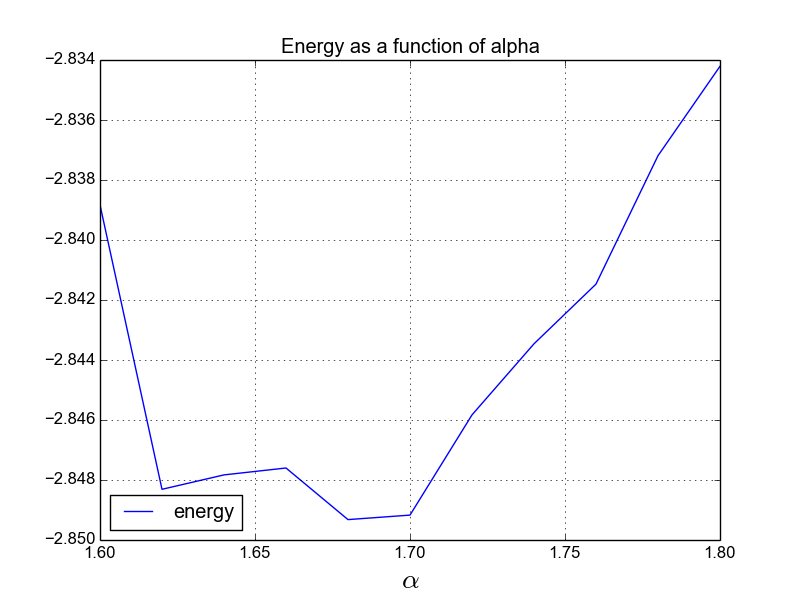
\includegraphics[width=0.8\textwidth]{../python_programs/EnergyVariance_helium2.png}
 	\label{Helium2}
 \end{figure}

 We now use Importance sampling in our calculations to look at which dt's are stable. 
 We can see from the plot below that using $dt = 10^-3$, we get stable results. A smaller $dt$ probably gives rise to different kinds of errors, like truncation errors etc.  
 \begin{figure}[H] 
 	\centering
 	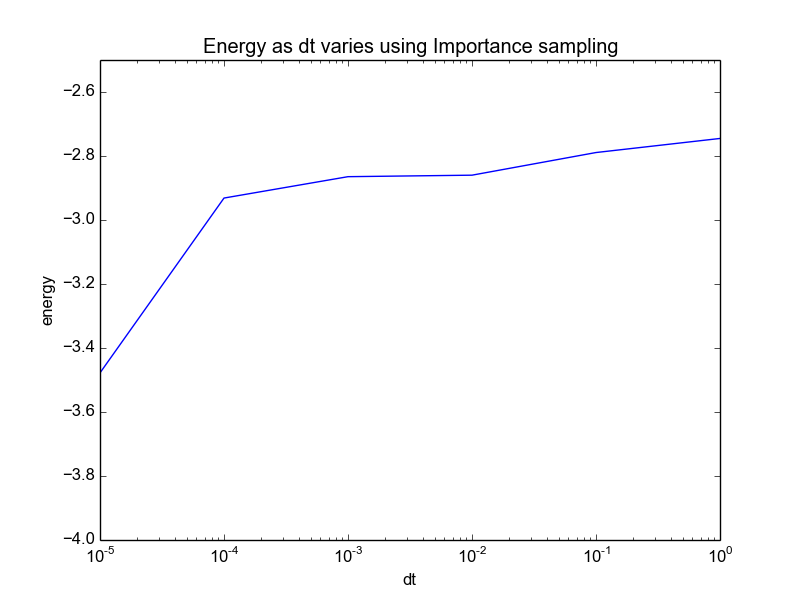
\includegraphics[width=0.8\textwidth]{../python_programs/ImportanceSampling_Helium_dt.png}
 \end{figure}

 We can also look at the effect of including the Jastrow factor. In the plot below, we see that we get noticably lower energies; Around $E = -2.89207$ for the optimal values of $\alpha$ and $\beta$. This plot does a poor job of representing which $\beta$ is optimal, but from now on, I will use the Steepest descent method to find the best $\beta$, so I will not use measurment by eyes to determine the beta. The best value I found in this plot was $\beta = 0.3$. 
 \begin{figure}[H]
 	\centering
 	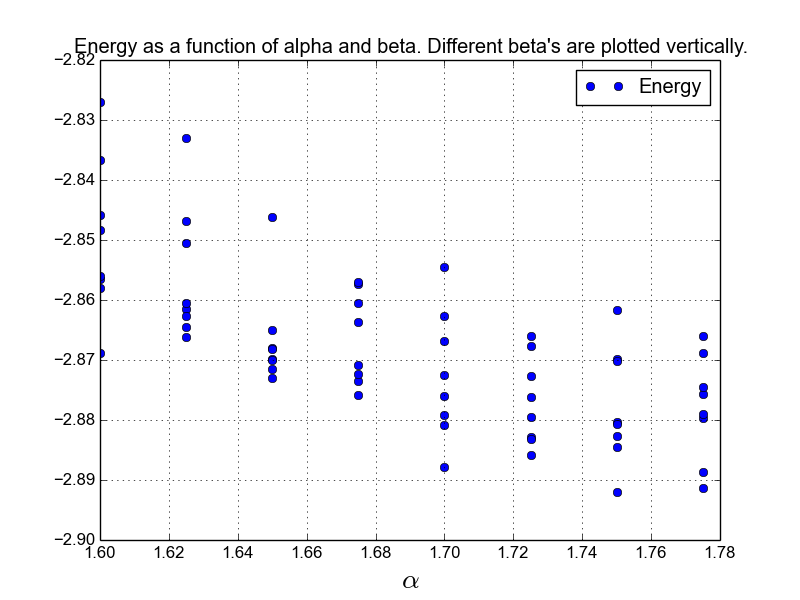
\includegraphics[width=0.8\textwidth]{../python_programs/EnergyVariance_helium5.png}
 	\label{Helium3}
 \end{figure}

 \end{subsection}
 \begin{subsection}{The Helium atom}
 	By excluding the Jastrow factor and the two-body potential in the local energy, one can test wether the Slater determinant is set up right. By setting $\alpha$ equal to the number of particles, one should get $E_0 = -4$. This can be reproduced, both with the analytical local energy, the numerical local energy, the numerical quantum force and the analytical quantum force. After doing these naive simulations, I include the Jastrow factor and the two-body potential. I will also use the method of steepest descent to find the optimal beta. This code runs in parallell and it is run using Importance sampling. The first results are produced without the Gaussian type orbitals. 

    \begin{figure}
 	\centering
 	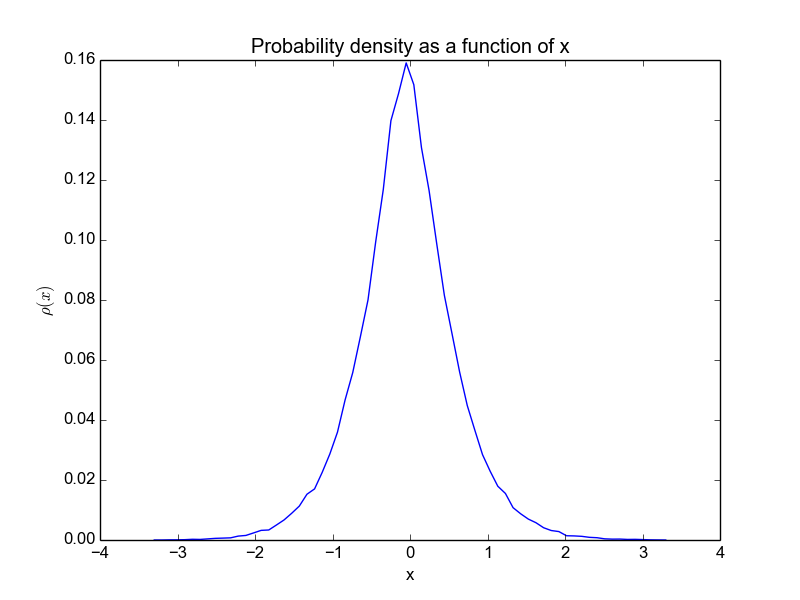
\includegraphics[width=0.8\textwidth]{../python_programs/ProbabilityDensity.png}
    \end{figure}
	 Since we only have the 1s-states, the density should be close in shape to the 1s-shape. This density will be more spread out when one take the electron-electron repulsion into account, because the repulsion can be seen as a reduction in the core's charge. 

	 By using the blocking analysis, the following plot shows how variance of the mean $E$-value changes when the block size changes. The y-axis shows the total error in the calculation. 
	 One see that the error is estimated to be around $0.29$. The spread seams to be pretty uniform and I conclude that the corrolation is low. 
	 \begin{figure}[H] 
	 	\centering
	 	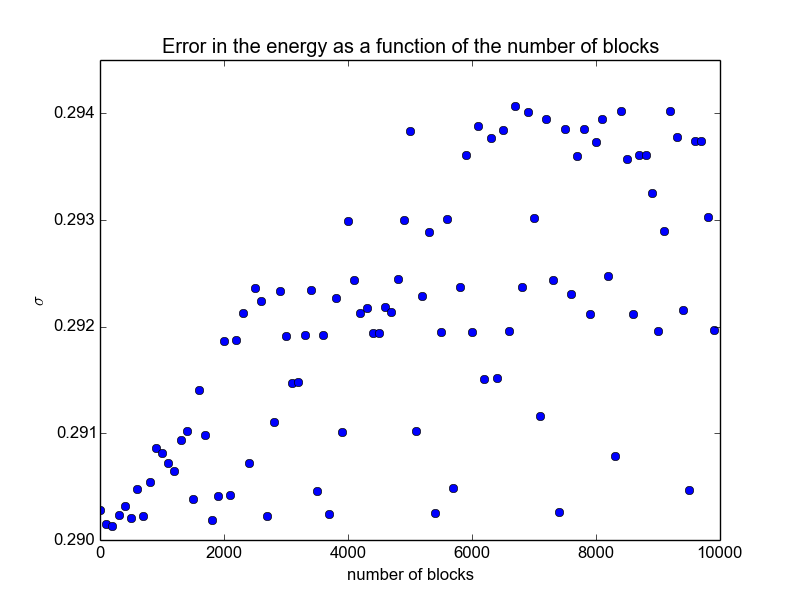
\includegraphics[width=0.8\textwidth]{../python_programs/HeliumBlocking.png}
	 \end{figure}

	 A short computation time comparison between the numerical and analytical gradients and Laplacians are found in the files, \textit{Helium\_CompareTime.txt}, \textit{Helium\_CompareTime\_ELnum.txt} and \textit{Helium\_CompareTime\_QFnum.txt}. All of them are done with Importance Sampling. 

	 We see that the results are about the same, but the time needed for the computation is $33$s for analytical, $52,3$s for the numerical local energy and finally $65.4$s for the numerical quantum force. 

	 For the final run on Helium with importance sampling and Steepest descent method, I set $\alpha = 1.75$ as I have seen that this alpha gave the lowest energy when the Jastrow factor was included. The steepest descent method stabilized at $\beta = 0.515163$. I used $10^7$ iterations for each core, so a total of $4 \cdot 10^7$ iterations in the calculation. This running is done with the Importance sampling method, so the only variational parameter that is not perfectly optimized is the value for $\alpha$. This can be fixed by including the Gaussian Orbitals which are a result of Hartree-Fock calculations. They do not have a parameter to be varied, and should for that reason give an optimal value. The result from this calculation is found in the file \textit{Helium\_final\_calculation.txt}. The result gained was
	 \begin{align*}
	 	E = -2.88538
	 \end{align*}
   	
    As the final calculation, I run the code in Project3\_Gaussian to do the calculations with Gaussian type orbitals. 
 \end{subsection}
 \begin{subsection}{The Beryllium atom}
 	Using the code in project 3 to do calculations on Beryllium. First I search for a good value of $\alpha$, looping through 20 different $\alpha$'s from 3 to 4.
 \begin{figure}
 	\centering
 	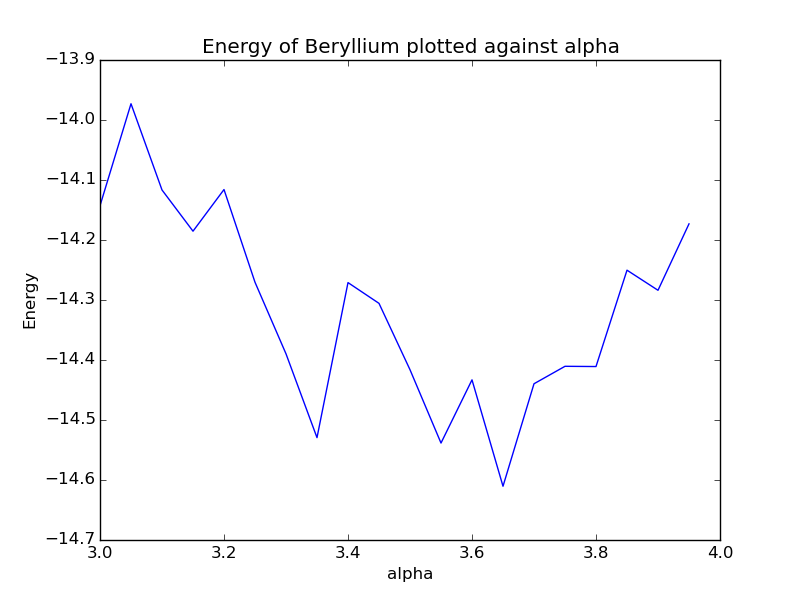
\includegraphics[width=\textwidth]{../python_programs/FindOptimalAlphaBeryllium.png}
 \end{figure}
 As seen in the figure, setting $\alpha = 3.65$ gives the lowest energy. A monte carlo integration with that alpha gives 
 \begin{align*}
 	E = -14.4144
 \end{align*}
 with $10^6$ iterations per core. The result is in the file \textit{Beryllium\_MC.txt}. Following is the one-body density ploted along with a blocking analysis show that the error lies around $3.7$. 
 \begin{figure}
 	\centering
 	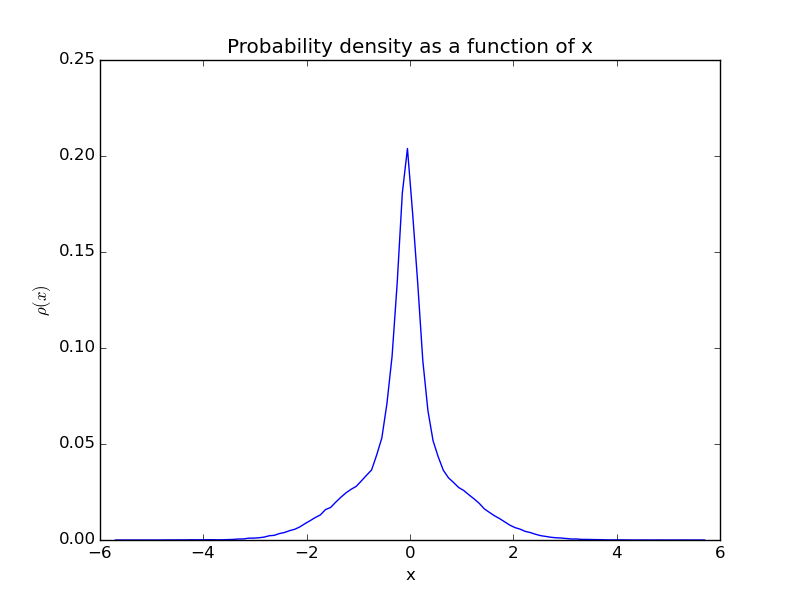
\includegraphics[width=\textwidth]{../python_programs/ProbabilityDensityBeryllium.png}
 	\caption{A plot showing the one-body density in the x-direction for a particle in the Beryllium atom}
 \end{figure}
 \begin{figure}
 	\centering
 	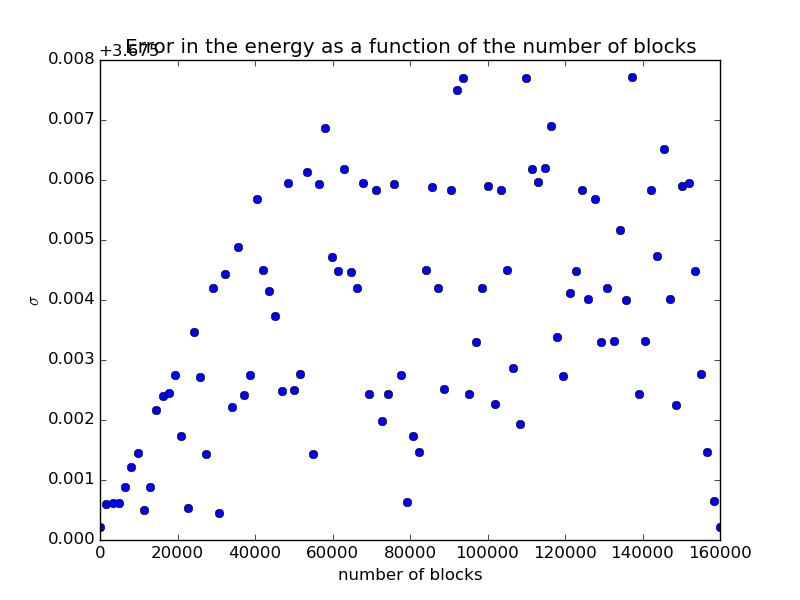
\includegraphics[width=\textwidth]{../python_programs/BerylliumBlocking.png}
 \end{figure}


 Unfortunatly the analytical computation of the quantum force does not give a satisfactory result when increasing particles above $2$, so the run with importance sampling is done with numerical differentiation. I did however not get as low energy with importance sampling as with the brute force Metropolis algorithm. The resulting energy for this computation was $E = -14.0801$. I plotted the one-body density for the brute force algorithm instead, because of a better calculation. The results from this calculation is found in \textit{Beryllium\_IS.txt}. 

 Running without the Jastrow factor, I surprisingly got a result close to the calculation with the factor. The energy was $E = -14.3423$. This is with the potential energy due to the repulsion between the electrons. Removing this repulsion, I get $E = -20$, which is expected. The results are found in \textit{Beryllium\_withoutJastrow.txt} and \textit{Beryllium\_withoutJastrow2.txt}. 
 \end{subsection}

 \begin{subsection}{The Neon atom}
 	
 \end{subsection}


\end{section}



\newpage

\appendix
\begin{section}{Appendix A}

\begin{subsection}{Analytical calculation of the local energy}
 Calculating the kinetic energy numerically is costly. One can considerably reduce computational time by using a closed form expression for the energy. 

 We have trial wavefunction 
 \begin{align*}
 	\Psi = e^{-\alpha(r_1 + r_2)}
 \end{align*}
 and we want to calculate the local energy given by
 \begin{align*}
 	E_L = \frac{1}{\Psi} \hat H \Psi
 \end{align*}
 where
 \begin{align*}
 	\hat H = -\frac{\nabla_1^2}{2} - \frac{\nabla_2^2}{2} - \frac{2}{r_1} - \frac{2}{r_2} + \frac{1}{r_{12}}
 \end{align*}
 Rewriting	
 \begin{align*}
 	T_{L1} = \frac{1}{\Psi} \left( -\frac{\nabla_1^2}{2} - \frac{\nabla_2^2}{2} \right) \Psi
 \end{align*}
 \begin{align*}
 	V_{L1} = \frac{1}{\Psi} \left( - \frac{2}{r_1} - \frac{2}{r_2} + \frac{1}{r_{12}} \right) \Psi
 \end{align*}
 Doing the calculations, we find that
 \begin{align*}
 	T_{L1} = -\frac{1}{2} \frac{1}{\Psi} \left( \frac{1}{r_1^2} \frac{\partial}{\partial r_1} \left( r_1^2 \frac{\partial}{\partial r_1} \Psi \right) + \frac{1}{r_2^2} \frac{\partial}{\partial r_2} \left( r_2^2 \frac{\partial}{\partial r_2} \Psi \right) \right)
 \end{align*}
 \begin{align*}
 	T_{L1} = -\frac{1}{2} \left( -\frac{2}{r_1}\alpha + \alpha^2 - \frac{2}{r_2} + \alpha^2 \right)
 \end{align*}
 Adding $T_{L1}$ and $V_{L1}$ 
 \begin{align*}
 	E_{L1} = \left( \alpha - 2 \right) \left( \frac{1}{r_1} + \frac{1}{r_2} \right) + \frac{1}{r_{12}} - \alpha^2 
 \end{align*}

 Introducing the Jastrow factor, one can rewrite the wavefunction
 as a product of the direct term and the corrolation term. 
 \begin{align*}
 	\Psi = \Psi_D \Psi_C
 \end{align*}
 We want to calculate the kinetic energy and divide by the wavefunction.
 \begin{align*}
 	T_{L2} = \frac{1}{\Psi} \frac{-\nabla^2}{2} \Psi
 \end{align*}
 Using the chain rule. This equation must be calculated for both particles. 
 \begin{align}
 	T_{L2} = -\frac{1}{2} \left( \frac{1}{\Psi_D}\nabla^2 \Psi_D + 2 \frac{1}{\Psi_D \Psi_C} \nabla \Psi_D \cdot \nabla \Psi_C + \nabla^2 \Psi_C \right)
 	\label{T_L2}
 \end{align}
 The first term is easily calculated, as it is the same as for $E_{L1}$
 \begin{align*}
 	\frac{1}{\Psi_D}\nabla^2 \Psi_D =  -\frac{2}{r_1}\alpha + \alpha^2 
 \end{align*}

 Calculating the second term
 \begin{align*}
 	\frac{1}{\Psi_D} \nabla \Psi_D = \frac{1}{\Psi_D} \frac{\partial}{\partial r} \Psi_D \hat e_r 
 \end{align*}
 \begin{align}
 	\frac{1}{\Psi_D} \nabla \Psi_D = -\alpha \hat e_r
 \end{align}
 When differentiating the corrolation term, given by
 \begin{align*}
 	e^{\frac{r_{12}}{2\left(1 + \beta r_{12} \right)}}
 \end{align*}
 One must use that
 \begin{align}
 	\frac{\partial}{\partial r_i} r_{12} = (-1)^{i+1} \frac{\vec r_1 - \vec r_2}{r_{12}} \hat e_{ri}
 \end{align}

 \begin{align*}
 	\frac{1}{\Psi_C} \nabla \Psi_C = \frac{1}{\Psi_C} \frac{\partial}{\partial r} \Psi_C \hat e_r 
 \end{align*}
 Giving for particle, $i$
 \begin{align*}
 	\frac{1}{\Psi_C} \nabla \Psi_C = (-1)^{i+1} \frac{\vec r_1 - \vec r_2}{2r_{12} \left(1+\beta r_{12} \right)}
 \end{align*}
 Finally multiplying and adding both particles. 
 \begin{align}
 	\frac{\nabla_1 \Psi_D}{\Psi_D} \cdot \frac{\nabla_1 \Psi_C }{\Psi_C} + \frac{\nabla_2 \Psi_D}{\Psi_D}  \cdot \frac{\nabla_2 \Psi_C}{\Psi_C}  = \frac{-1}{\left(1+\beta r_{12} \right)} \left( \frac{\alpha(r_1 + r_2)}{r_{12}} \left(1 - \frac{\vec r_1 \cdot \vec r_2)}{r_1 r_2} \right)  \right)
 \end{align} 

 Now, to calculate the last term in (\ref{T_L2}). 
 \begin{align}
 	\frac{\nabla^2 \Psi_C}{\Psi_C} = \frac{1}{\Psi_C} \left( \frac{2}{r} \frac{\partial}{\partial r}\Psi_C + \frac{\partial^2 }{\partial r^2} \Psi_C \right)
 \end{align}
 Looking at the first part for both particles
 \begin{align*}
 	\frac{2}{r_1} \frac{\vec r_1 - \vec r_2}{2r_{12} \left(1+\beta r_{12} \right)} \frac{\vec r_1}{r_1} + \frac{2}{r_1} \frac{\vec r_2 - \vec r_1}{2r_{12} \left(1+\beta r_{12} \right)} \frac{\vec r_2}{r_2}
 \end{align*}
 Sorting this gives
 \begin{align*}
 	\frac{2}{r_{12}(1+\beta r_{12})^2} - \frac{\vec r_1 \cdot \vec r_2}{r_{12} r_1^2 (1 +\beta r_{12})^2} - \frac{\vec r_1 \cdot \vec r_2}{r_{12} r_2^2 (1+\beta r_{12})^2}
 \end{align*}
 The second part for particle 1
 \begin{align*}
 	\frac{1}{\Psi_C} \frac{\partial^2 }{\partial r^2} \Psi_C = \left( \frac{\vec r_1 - \vec r_2}{2r_{12} \left(1+\beta r_{12} \right)} \hat e_{r1} \right)^2 + \frac{\partial}{\partial r_1} \left( \frac{\vec r_1 - \vec r_2}{2r_{12} \left(1+\beta r_{12}  \right)} \hat e_{r1} \right) 
 \end{align*}
 \begin{align*}
 	\frac{1}{4(1+\beta r_{12})^4} + \frac{\beta}{(1+\beta r_{12})^3}
 \end{align*}
 Combining these calculations
 \begin{align*}
 	 \frac{\nabla^2 \Psi_C}{\Psi_C} = \frac{1}{r_{12}(1+\beta r_{12})^2} + \frac{1}{4(1+\beta r_{12})^4} - \frac{\beta}{(1+\beta r_{12})^3}
 \end{align*}
 Combining, we get the $T_{L2}$
 
 Giving the total local energy
 \begin{align*}
 	E_{L2} = E_{L1} + \frac{1}{2(1+\beta r_{12})^2} \left[ \frac{\alpha (r1+r2)}{r_{12}} \left(1 - \frac{\vec r_1 \cdot \vec r_2}{r_1 r_2} \right) - \frac{1}{2(1+\beta r_{12})^2} - \frac{2}{r_{12}} + \frac{2 \beta}{1 + \beta r_{12}} \right]
 \end{align*}

 More general expressions are used in the code in Project 3. 
 \end{subsection}
 \end{section}


\end{document}